\subsection{Differensforstærker}
\label{effekt_differensforstaerker}

\begin{figure}[h]
\centering
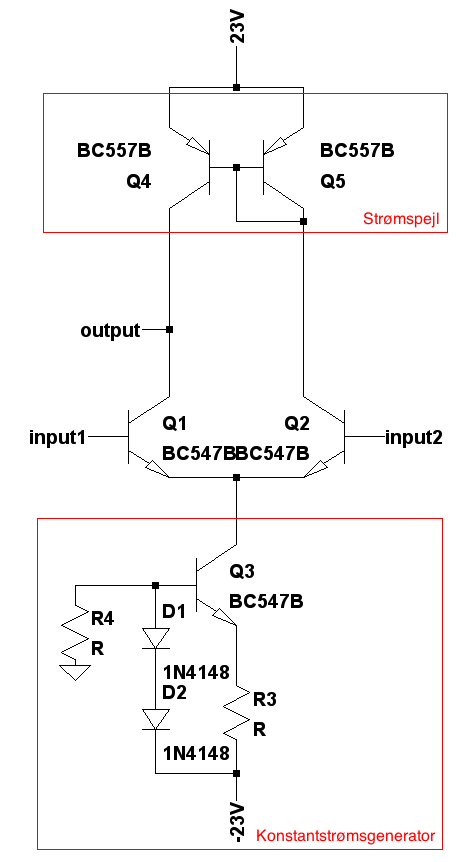
\includegraphics[scale=.4]{teknisk/effektforstaerker/differensforstaerker.png}
\caption{Diagram over differensforstærkeren hvor strømspejl og konstantstrømsgenerat er markeret}
\label{fig:differensforstaerker}
\end{figure}

Differensforstærkerens formål er at danne platform for en tilbagekobling ved at forstærke forskellen mellem signalet på input1 og input2 samt undertrykke common-mode signaler. Strømgeneratoren sørger for at der løber en konstant strøm, $\frac{1}{2}I_\mathrm{bias}$, i de to grene af differensforstærkeren når input1 = input2. For at disse strømme effektivt skal være ens er det nødvendigt at benytte matchede transistorer til både strømspejlet og Q1 og Q2. Stiger strømmen gennem Q2 med $\Delta I$, som følge af en øget spænding på input2 relativt til input1, vil strømspejlet øge strømmen i den modsatte gren så strømmene i de to grene er ens. Da der nu løber $\frac{1}{2}I\mathrm{bias} + \Delta I$ i begge grene, men kun kan løbe $I_\mathrm{bias}$ gennem konstantstrømsgenerator vil der nødvendigvis løbe $I_\mathrm{bias} -\Delta I$ gennem Q1 og $2\Delta I$ ud i outputgrenen. Denne sammenhænge gælder både med en strømforøgelse og -formindskelse gennem Q2. På denne måde styres spændingsforstærkeren, som er dokumenteret i afsnit \ref{effekt_spaendingsforstaerker}. 

Biasstrømmen, $I_\mathrm{bias}$, som konstantstrømsgeneratoren skal generere vælges til 2 mA, da transistorparametrene for den anvendte transistor, BC547b (Q3), er veldefinerede ved denne collectorstrøm, hvilket letter beregningerne. Når der løber en strøm gennem generatoren på 2 mA vil der, hvis differensforstærkeren er i balance, løbe 1 mA i hver gren. Der antages at transistorparametrene angivet ved en collectorstrøm på 2 mA også er gældende for en strøm på 1 mA. 
Konstantstrømsgeneratoren designes ud fra samme procedure som benyttes i underafsnittet Konstantstrømsgenerator i afsnit \ref{effekt_stroemforstaerker}. $I_F$ aflæses i databladet for 1N4148 til 5 mA hvis en $V_F$ på 700 mV, hvilket er den nødvendige $V_\mathrm{be}$ for Q3 for at opnå en collectorstrøm på 2 mA. Med denne procedure bliver strømgeneratorens komponentværdier som vist i ligning (\ref{eq:stroemdiff1}) og (\ref{eq:stroemdiff2}).

\begin{equation}
\label{eq:stroemdiff1}
R_4=\frac{23~\mathrm{V}-2 \cdot 0,7~V}{5~\mathrm{mA}}=4,32~\mathrm{k}\ohm
\end{equation}

\begin{equation}
\label{eq:stroemdiff2}
R_3=\frac{0,7~\mathrm{V}}{2~\mathrm{mA}}=350~\ohm
\end{equation}

For at kunne beregne CMRR, som er et udtryk for forholdet mellem differensforstærkningen og common-mode-forstærkningen, er der behov for netop at beregne disse forstærkninger. 
Differensforstærkningen, $A_d$, er et udtryk for hvor meget spændingsdifferensen mellem inputsignalet og det tilbagekoblede signal forstærkes. I ligning \ref{eq:diffforstaerkning} er der 


\subsubsection*{Simulering}